\documentclass{cumcm}


% \title{text}这里是显示在第三页的文章标题
\title{机场的出租车问题}
% \displaytitle{text} 这里是显示在承诺书上的文章标题,注意,不能换行,如果题目特别长,要进行适当的缩写
\displaytitle{机场的出租车问题}
% \school{text}命令用于在承诺书上显示学校名称。按要求,此处应填写全称
\school{上海交通大学}
% 以下命令分别显示队员、指导教师姓名以及队伍编号
\authorone{刘畅}
\authortwo{谢哲}
\authorthree{胡胜超}
\advisor{}
\teamnumber{未知报名号}
\dateyear{2019}
\datemonth{9}
\dateday{7}

\begin{document}

% 这里用于打印承诺书以及编号页
 
%\newpage
\thispagestyle{empty} %取消当前页码
{\Large \heiti \begin{center}\the\year~高教社杯全国大学生数学建模竞赛\par\vspace{0.5\ccwd}\par
{\ziju{1}承诺书}\end{center}\par\vspace{1\ccwd}\par}
\renewcommand{\baselinestretch}{1.5}\normalsize
{\zihao{-4}%
我们仔细阅读了中国大学生数学建模竞赛的竞赛规则。\par
我们完全明白,在竞赛开始后参赛队员不能以任何方式(包括电话、电子邮件、网上咨询等)
与队外的任何人(包括指导教师)研究、讨论与赛题有关的问题。\par
我们知道,抄袭别人的成果是违反竞赛规则的, 如果引用别人的成果或其他公开的资料
(包括网上查到的资料),必须按照规定的参考文献的表述方式在正文引用处和参考文献中明确列出。\par
我们郑重承诺,严格遵守竞赛规则,以保证竞赛的公正、公平性。如有违反竞赛规则的行为,我们将受到严肃处理。\par
\par\vspace{2\ccwd}\par
\raisebox{1ex}[0pt]{我们参赛的题目是:}\vbox{\hbox to11.4cm{\hfil \the\displaytitle \hfil}
        \protect\vspace{0.6truemm}\relax
        \hrule depth0pt height0.15truemm width11.4cm}\par
\vspace{1mm}
\raisebox{1ex}[0pt]{我们的参赛报名号为(如果赛区设置报名号的话):}\vbox{\hbox to5.75cm{\hfil \the \teamnumber  \hfil}
        \protect\vspace{0.6truemm}\relax
        \hrule depth0pt height0.15truemm width5.75cm}\par
\vspace{1mm}
\raisebox{1ex}[0pt]{所属学校(请填写完整的全名):}\vbox{\hbox to9.12cm{\hfill \the\school \hfill}
        \protect\vspace{0.6truemm}\relax
        \hrule depth0pt height0.15truemm width9.12cm}\par
\begin{tabular}{lcp{8.82cm}c}
\hspace{-2.1mm}\raisebox{-1mm}[0pt]{参赛队员(打印并签名): }&\raisebox{-1mm}[0pt]{1、}& \raisebox{-1mm}[0pt]{\the\authorone\hfill{}}& \\ \cline{3-3}
   &\raisebox{-1mm}[0pt]{2、}& \raisebox{-1mm}[0pt]{\the\authortwo\hfill{}}& \\ \cline{3-3}
   &\raisebox{-1mm}[0pt]{3、}& \raisebox{-1mm}[0pt]{\the\authorthree\hfill{}}& \\ \cline{3-3}
\end{tabular}
\par
\vspace{10mm}
\raisebox{1ex}[0pt]{指导教师或指导教师组负责人(打印并签名):}\vbox{\hbox to6.65cm{\the\advisor \hfil}
        \protect\vspace{0.6truemm}\relax
        \hrule depth0pt height0.15truemm width6.65cm}\par
\vspace{5mm}
{}\hspace{10cm}日期:\uline{\hspace{0.5em}\the\dateyear\hspace{0.5em}}年\uline{\hspace{0.5em}\the\datemonth\hspace{0.5em}}月 
\uline{\hspace{0.5em}\the\dateday\hspace{0.5em}}  日
\par
\vspace{2cm}
\hrulefill\par\vspace{2\ccwd}\par
赛区评阅编号(由赛区组委会评阅前进行编号):
}
\renewcommand{\baselinestretch}{1.3}\normalsize
\newpage
\thispagestyle{empty} %取消当前页码
{\Large \heiti \begin{center}\the\year~高教社杯全国大学生数学建模竞赛\par\vspace{0.5\ccwd}\par
{\ziju{1}编号专用页}\end{center}\par\vspace{1\ccwd}\par}
{\zihao{-4}%
\par\vfill
赛区评阅编号(由赛区组委会评阅前进行编号):\par\vfill\vfill

赛区评阅记录(可供赛区评阅时使用):\vspace{1\ccwd}

\begin{center}
\resizebox{.9\textwidth}{!}{
\begin{tabular}{|c|*{10}{p{.09\textwidth}|}}
\hline
\makecell{评\\阅\\人}&&&&&&&&&&\\
\hline
\makecell{评\\分}&&&&&&&&&&\\
\hline
\makecell{备\\注}&&&&&&&&&&\\
\hline
\end{tabular}
}
\end{center}\vspace{1\ccwd}

全国统一编号(由赛区组委会送交全国前编号):\par\vfill\vfill

全国评阅编号(由全国组委会评阅前进行编号):\par\vfill\vfill\vfill
}
\renewcommand{\baselinestretch}{1.3}\normalsize

\newpage

\begin{minipage}{0.9\textwidth}
\centering\LARGE\textbf{机场的出租车问题}
\end{minipage}

% 摘要和关键字
\begin{abstract}
	摘要部分,是文章最为重要的部分之一,一般放在最后来写。
	引用一些参考文献。首先简要概括一下题目。\par
	\textbf{针对问题一}\quad
	对问题一的解答的概括。\par
	\textbf{针对问题二}\quad
	对问题二的解答的概括。\par
	\textbf{针对问题三}\quad
	对问题三的解答的概括。
\\\par
\textbf{关键词\quad MATLAB\quad \LaTeX}
\end{abstract}

\newpage
\section{问题重述}
\subsection{问题背景}
出租车是乘客往返市区与机场的主要交通方式之一。机场有客流密度大的特点,而乘客需要在固定的出租车上客点乘车。由于上客点地点和条件有限,且上客的效率受到了乘客、机场航班、出租车司机等多种因素的影响。所以需要一种优化的解决方案能够提高乘客在出租车上客点的乘车效率,以减少乘客和出租车司机的等待时间。
\subsection{问题重述}
国内机场一般将出租车乘车区分为上客区和下客区两个分开的区域,并且对于离开上客区的出租车,司机可以根据的意愿选择放空车辆直接离开或前往“蓄车池”载客。对于司机,他们可以得到当前“蓄车池”内的车的数量以及当前的航班数量来决定是否进入“蓄车池”等待,并且司机通常还可以根据自己的经验,结合季节、时间等因素判断乘客数量的多少。如果司机选择直接放空返回,则可能会有返回时的空载费用和载客的潜在收益的损失。对于机场管理者,他们需要在上客地点的等候区采取“分批定量”放行的措施来让乘客依次进入上客区乘车。\par
\begin{figure}[H]
	\centering
	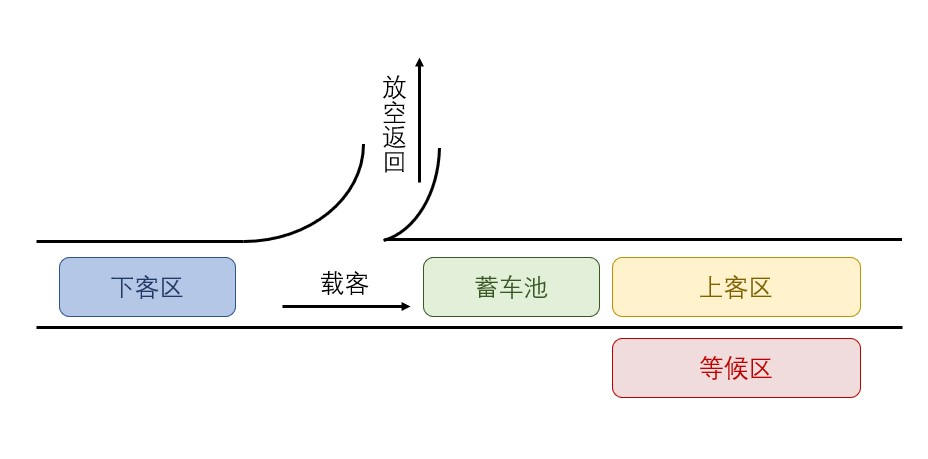
\includegraphics[width=1.0\textwidth]{img/taxi_example.jpg}
	\caption{机场出租车乘车区域示意图}
	\label{taxi_example}
\end{figure}
根据以上条件,我们需要研究如下的4个问题:
\begin{enumerate}[(1)]
	\item 建立一个模型,用于出租车司机载客与放空返回的选择策略。建立模型时综合考虑机场在不同时间的旅客数量的变化规律和其它的相关因素,使得出租车的做出的策略能够使其收益最大化。
	\item 获取国内某一机场的实际数据,根据建立的模型和机场的实际数据计算出司机的决策策略,并由此可以出模型的合理性与对相关因素的依赖程度。
	\item 机场乘车区设置有两条并行车道,建立一个模型,确定合理的“上车点”的位置,与出租车和乘客的安排方式,在确保安全的前提下,使得出租车和乘客的乘车效率能够最大化。
	\item 出租车在机场载客的目的地不确定,且司机无法自主选择载客或拒绝载客,故司机的收益不确定。为了解决这个问题,考虑给予返回的短途载客的司机在下一次载客时的优先权。建立一个模型,给出可行的优化方案,使得出租车司机们的收益能够尽可能均衡。
\end{enumerate}

\section{模型假设}
\begin{enumerate}
	\item 考虑到每个人上车的时间相差较小,可以认为每个人从乘车区上车到出租车起步离开的时间固定,我们记这个时间为$t_0$。
	\item 本文认为在我们考虑的一段时间之内,航班到达机场的时间分布是均匀的。
	\item 在一段时间之内,各个航班到达的乘客前往出租车乘车区域乘车的人数符合泊松分布。
	\item 每一个到达航班的需要乘坐出租车的乘客到达出租车乘车等候区的时间满足泊松分布。
	\item 由于汽车在等待时由于仍在运行中,其耗油量近似为正常运行时的$\frac{1}{2}$,所以可以认为出租车在“蓄车池”等待期间消耗的油量较正常运行时更低。
\end{enumerate}

% 符号变量设置
\newcommand{\flightnum}{$N_f$}
\newcommand{\taxinum}{$N_c$}
\newcommand{\waittime}{$t_w$}

\section{符号说明}
表\ref{table-symbol}列出了本文需要的符号。
\begin{table}[H]
	\centering
	\caption{符号说明} 
	\label{table-symbol}
	\begin{tabular*}{0.65\textwidth}{ccc}
		\toprule
		符号 & 意义 & 单位 \\
		\midrule
		\flightnum & 一段时间内的航班数量 & 架 \\
		\taxinum & 蓄车池内的出租车数量 & 辆 \\
		$T$ & 模型考察的总时间长度 & $min$ \\
		\waittime & 出租车司机等待的时间 & $min$ \\
		$t_r$ & 出租车从机场返回市区的时间 & $min$ \\
		$n_i$ & 第$i$架航班上需要乘坐出租车的人数 & 人 \\
		$M_0$ & 一架航班乘坐出租车的人数最大值 & 人 \\
		$\Delta t_f$ & 航班的时间间隔 & $min$ \\
		$p_i$ & 第$i$架航班乘客乘坐出租车的概率 & \\
		$q_i$ & 第$i$架航班乘客抵达候车区的时间分布 & \\
		$\lambda_1$ & 航班乘坐出租车人数分布的均值 & \\
		$\mu$ & 乘客到达乘车区时间正态分布均值 & \\
		$\sigma$ & 乘客到达乘车区时间正态分布标准差 & \\
		$N$ & 开始时蓄车池内出租车能够容纳的乘客人数 & 人 \\
		$\overline{t_0}$ & 平均每辆车上车所需耗费时间 & $min$ \\
		$t_1$ & 到达等候区乘客累计达到$N$的时刻 & $min$ \\
		$t_2$ & 载客出租车返回市区的时刻 & $min$ \\
		$t_{extra}$ & 出租车额外等待的时间 & $min$ \\
		$\varepsilon_0$ & 平均每辆车的载客数 & 人$/$辆 \\
		$E_1$ & 每辆出租车从空载返回到$t_2$时刻的利润 & 元 \\
		$E_2$ & 每辆出租车从进入蓄车池到$t_2$时刻的利润 & 元 \\
		$\overline{E_o}$ & 出租车正常行驶平均每分钟油费 & 元$/min$ \\
		$\overline{E_{wo}}$ & 出租车排队时平均每分钟油费 & 元$/min$ \\		$\overline{E_i}$ & 出租车在市区内运营平均收入 & 元$/min$ \\
		$\overline{E_c}$ & 出租车平均载客返回收入 & 元 \\
		\bottomrule
	\end{tabular*}
\end{table}

\section{问题分析}
\subsection{问题一的分析}
问题一的本质就是要建立一个出租车司机关于一段时间内航班数量\flightnum 与当前蓄车池内出租车的数量\taxinum 的决策模型$f\left(\mbox{\flightnum},\mbox{\taxinum}\right)$,而这个模型可以分成如下的两个部分:
\begin{enumerate}[(1)]
	\item 出租车时间等待时间$t$与航班数量\flightnum 和蓄车池内出租车数量\taxinum 的预测模型$\mbox{\waittime}\left(\mbox{\flightnum},\mbox{\taxinum}\right)$,通过计算机模拟的方法,得出可行域内的不同\flightnum 和\taxinum 下的\waittime 的数值,可以绘制出\waittime 关于\flightnum 和\taxinum 的函数关系图像。
	\item 建立数学模型,得到出租车不载客利润$E_1$和出租车载客利润$E_2$与出租车等待时间\waittime 之间的函数关系$E_1(\mbox{\waittime})$和$E_2(\mbox{\waittime})$,并做出出租车司机的决策$\max(E_1(\mbox{\waittime}),E_2(\mbox{\waittime}))$,由此得到出租车司机关于等待时间的决策函数$E(\mbox{\waittime})$。
\end{enumerate}
\par
将如上的两个数学模型得到的函数$t\left(\mbox{\flightnum},\mbox{\taxinum}\right)$和$E(\mbox{\waittime})$联立,最终得到出租车司机关于\flightnum 和\taxinum 的决策函数$f(\mbox{\flightnum},\mbox{\taxinum})$。

\subsection{问题二的分析}
问题二的本质是需要根据搜集国内的某一个机场的实际数据,带入问题一中得到的模型,得到不同条件下出租车司机的最佳选择策略,由此对问题一中的模型进行数值上的验证,所以问题二的解决需要分为如下几个步骤:
\begin{enumerate}[(1)]
	\item 收集国内某一城市的机场航班数量分布情况、出租车出入场、场内出租车数量、该城市机场到市区出租车均价、单位时间油耗价格和出租车单位时间正常收入。
	\item 根据收集到的数据,带入问题一中建立的模型,计算出租车司机等待时间的阈值$t_{w0}$。
	\item 根据收集到的参数,绘制出$t_w-N_f,N_c$图像,作平面$\alpha:t_w=t_{w0}$,得到平面$\alpha$和$t_w$平面的交线$l:\alpha\cap t_w(N_f,N_c)$,则$l$即为$t_w$的阈值曲线。
	\item 根据收集到的数据,随机抽取部分数据,带入上述模型进行计算,得到预计的等待时间$\hat{t_w}$,与实际的等待时间进行比较,分析模型的误差和对相关因素的敏感程度。
\end{enumerate}

\subsection{问题三的分析}
问题三要求给出一个合理的乘客“上车点”设置方式,在保证安全的前提之下,能够降低乘客的平均等待时间。
\subsection{问题四的分析}

\section{模型建立}
针对本题,本文一共建立了三个数学模型:用于出租车司机决策的模型、用于设置机场停车点的模型、用于短途载客返回出租车优先权的模型。下面依次对这三个模型的建立作详细说明。
\subsection{用于出租车司机决策的模型}
用于出租车司机决策的模型一共分为出租车等待时间$\mbox{\waittime}\left(\mbox{\flightnum},\mbox{\taxinum}\right)$和出租车司机决策$E(\mbox{\waittime})$两个部分,以下依次描述这两个模型的具体建立过程,并将两个模型综合得到最终的决策模型。
\subsubsection{出租车等待时间}
乘客在乘车区排队等待出租车采用排队论中$M/G/1/\infty/N/FCFS$模型进行分析。出租车的等待时间分为两部分,一部分是乘客上车占用的时间$Bt_0$,另一部分是由于乘坐出租车的乘客前往乘车点的时间间隔过大,导致的出租车空闲等待的时间:
\begin{equation}
	t_{extra}=\sum_it_{extrai}
	\label{eq:textrafunc}
\end{equation}
由此可以得到等待时间\waittime 的计算公式:
\begin{equation}
	\mbox{\waittime}=\mbox{\taxinum}\overline{t_0}+t_{extra}
	\label{eq:tfunc}
\end{equation}
\par
航班的之间的间隔$\Delta t_f$与总时间$T$和航班数目\flightnum 满足如下的关系:
\begin{equation}
	\Delta t_f=T/\mbox{\flightnum}
	\label{eq:deltatf}
\end{equation}
对于一段时间内航班到达的数量分布,本文认为其满足均匀分布的规律。其中,对于每一架航班乘坐出租车的人数$n_i$,其与每一架航班乘坐出租车的最大人数$M_0$和该架航班上的乘客乘车概率$p_i$满足如下关系:
\begin{equation}
	n_i=M_0·p_i
	\label{eq:passengernum}
\end{equation}
由此,我们可以通过公式\ref{eq:passengernum}来确定不同时间段到达机场的乘客的数量,对于概率$p_i$,本文认为其满足均值为$\lambda_1$的泊松分布:
\begin{equation}
	p_i(X=k)=\frac{\lambda_1}{k!}e^{-\lambda_1}
	\label{eq:pi}
\end{equation}
对于进入等候区排队的乘客,考虑使用排队论中的模型。其中对于每一架到达的航班,从航班到达,至需要乘坐出租车的乘客抵达出租车等候区排队的时间,本文认为其关于时间的分布满足均值为$\mu$,标准差为$\sigma$的正态分布:
\begin{equation}
	q_i((i-1)\Delta t_f+t)=\frac{1}{\sqrt{2\pi}\sigma}e^{-\frac{(t-\mu)^2}{2\sigma^2}},\quad t\ge0
	\label{eq:qi}
\end{equation}
对于此时在蓄车池中的车辆数量,其数量\taxinum 与能够承载的乘客人数$N$满足如下关系:
\begin{equation}
	N=\mbox{\taxinum}·\varepsilon_0
	\label{eq:N}
\end{equation}
根据以上描述的符号关系,与式\ref{eq:N}联立,我们可以列出承载乘客与到达乘客的关系:
\begin{equation}
	\sum_i\int_0^{t_1}M_0\cdot p_iq_i(t)\mathrm{d}t=\mbox{\taxinum}\cdot\varepsilon_0
\end{equation}
\subsubsection{出租车收益与等待时间关系}
出租车的收益可以分为空再返回和等待载客两部分进行分别分析。分析的时间段为出租车下客完成(时间起点),至载客返回的出租车抵达市区的时间$t_2$。
\begin{enumerate}[(1)]
	\item \textbf{空载返回出租车收益。}\par
	空载返回的出租车由于无需等待,所以其能够在空载返回市区后直接载客运营,故空载返回的出租车的收入为其在市区运营时的收入,其耗费为全程的油费。于是我们可以得到如下空载返回出租车收益$E_1$关于$t_2$的关系:
	\begin{equation}
		E_1(t_2)=\overline{E_i}\cdot(t_2-t_r)-\overline{E_o}\cdot t_2
		\label{eq:E1}
	\end{equation}
	\item \textbf{载客出租车收益。}\par
	由于载客出租车需要在蓄车池内等待乘客,而根据假设,蓄车池内等待不消耗任何成本,所以载客出租车的收入为载客从机场返回市区的收入,消耗为返回市区时的油耗。于是我们可以得到如下空载返回出租车的收益$E_2$的表达式:
	\begin{equation}
		E_2=\overline{E_c}-t_r\cdot\overline{E_o}-t_2\cdot\overline{E_{wo}}
		\label{eq:E2}
	\end{equation}
\end{enumerate}
\par
此外,我们还可以得到出租车等待时间\waittime 和载客出租车返回市区的时间$t_2$时间的关系:
\begin{equation}
	t_2=\mbox{\waittime}+t_r
	\label{eq:t2}
\end{equation}
将式\ref{eq:E1}、\ref{eq:E2}、\ref{eq:t2}联立,我们可以得到用于司机决策的\waittime 的阈值,由此建立用于出租车司机决策的模型。
\subsection{用于设置机场停车点的模型}

\subsection{用于短途载客返回出租车优先权的模型}

\section{问题解答}
\subsection{问题一的解答}
对于问题一,本文建立了出租车司机的决策模型。这个模型分为出租车等候时间和出租车收益两个部分,根据以上建立的模型分别对这两个模块进行求解。\par
对于出租车等候时间,在选定的时间范围之内,建立了航班到达、乘客前往乘车区,和乘客在乘车区排队上车的模型,即出租车的等待时间\waittime 关于航班数量\flightnum 和蓄车池内出租车数量\taxinum 的函数关系,并使用如图\ref{fi:program1}所示的程序模拟了这一过程。
\begin{figure}[H]
	\centering
	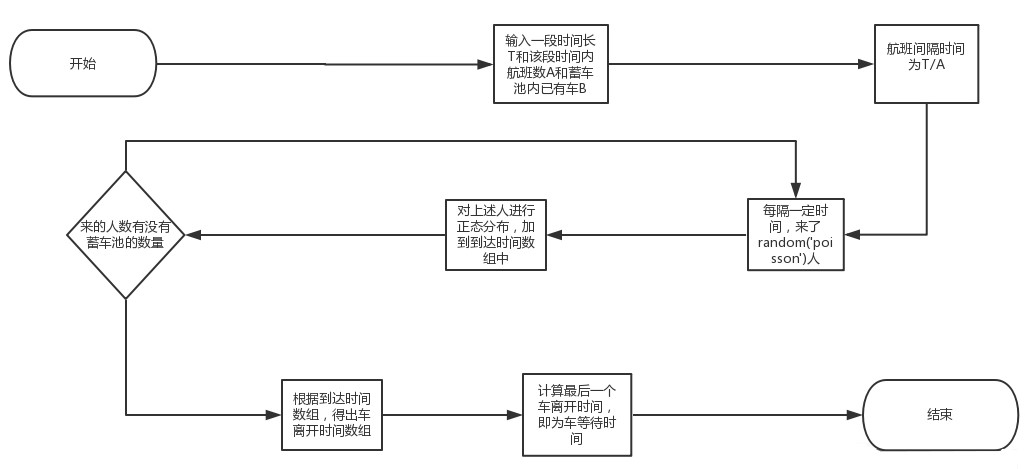
\includegraphics[width=0.8\textwidth]{img/program1.jpg}
	\caption{出租车等待时间模拟程序框图}
	\label{fi:program1}
\end{figure}
\par
该计算机程序的算法的运行主要分为如下几个步骤:
\begin{enumerate}[(1)]
	\item 程序接收输入的两个数据:一段时间内的航班数量\flightnum 和此时蓄车池内的出租车数量\taxinum ,由此计算出航班之间的间隔时间。
	\item 当每一架航班到达时,程序调用random函数根据泊松分布的规律,计算出每一架航班的人数。
	\item 将每一架航班到达的人数按照正态分布的时间规律,加入到不同时间段内的人数的数组中,实现排队队列的模拟功能。直到到达队列中的人数达到蓄车池内的出租车能够容纳的人数$N$为止,结束循环。
	\item 模拟一个队列,将各个时间的排队的数量依次加入乘车队列中,与此同时蓄车池内的出租车按照一定的时间间隔进行载客。最后计算整个过程花费的时间,并输出结果。
\end{enumerate}
通过运行如图所示的程序,我们得到了不同条件下的出租车司机需要等待的时长。取不同的\flightnum 和\taxinum 的值,输入程序,可以得到如图\ref{fi:problem1func}所示的函数图像。
\begin{figure}[H]
	\centering
	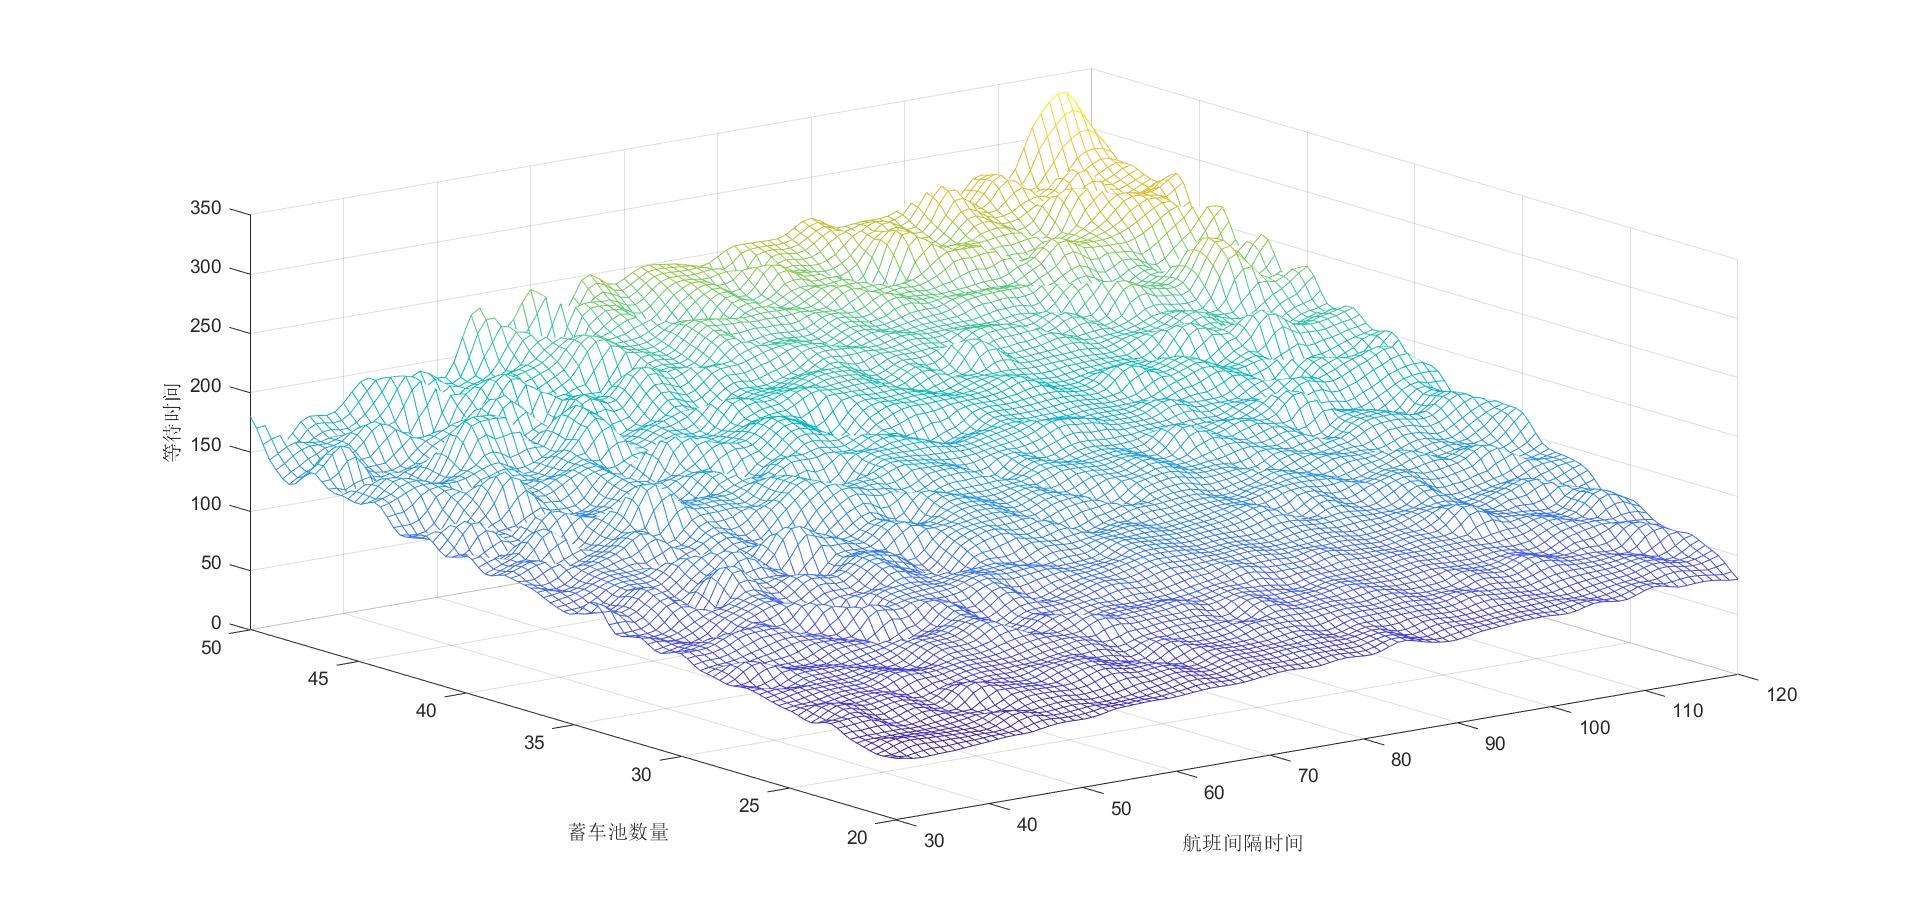
\includegraphics[width=1.0\textwidth]{img/problem1_func.jpg}
	\caption{\waittime$(\mbox{\flightnum,\taxinum})$函数图像}
	\label{fi:problem1func}
\end{figure}
\par
对于出租车收益,通过联立式\ref{eq:E1}、式\ref{eq:t2}和式\ref{eq:E2}可以得到等待时间\waittime 的分界值:
\begin{equation}
	\mbox{\waittime}_0=\frac{\overline{E_c}-\overline{E_{wo}}\cdot t_r}{\overline{E_t}-\overline{E_o}+\overline{E_{wo}}}
	\label{eq:tw}
\end{equation}
\par
综上所述,根据如下关系,可以得出出租车司机的最佳决策:
\begin{equation}
	\begin{cases}
		\mbox{  空载返回} &  \mbox{\waittime}(\mbox{\flightnum,\taxinum})\ge\mbox{\waittime}_0 ,\\
        \mbox{  等待载客} &  \mbox{\waittime}(\mbox{\flightnum,\taxinum})<\mbox{\waittime}_0  .
	\end{cases}
\end{equation}
\subsection{问题二的解答}
对于问题二,我们从各种渠道收集了关于国内某城市的机场和出租车的多种数据,用于对问题一中建立的模型进行正确性的分析与评估。\par
\begin{enumerate}[(1)]
	\item \textbf{出租车等待时间阈值计算。}\par
	我们收集了问题一中的模型中所需要的基本数据,这些数据在表中列出。
	\begin{table}[H]
		\centering
		\caption{城市出租车基本数据\cite{taxidata,taxireport}} 
		\label{table-symbol}
		\begin{tabular*}{0.31\textwidth}{ccc}
			\toprule
			项目 & 值 & 单位 \\
			\midrule
			平均车速 & 31.23 & $km/h$ \\
			空驶率 & $21.13\%$ & \\
			单价 & 1.82 & 元$/km$ \\
			油费 & 0.54 & 元$/km$ \\
			$\overline{E_c}$ & 62 & 元 \\
			$t_r$ & 50 & min \\
			\bottomrule
		\end{tabular*}
	\end{table}
	根据这个表格,可以计算出单位时间出租车平均收入$\overline{E_t}=0.75\mbox{元}/min$,单位时间出租车正常行驶平均油费$\overline{E_o}=0.28\mbox{元}/min$,排队中出租车单位时间平均油费$\overline{E_{wo}}=0.14\mbox{元}/min$。将该数据与上表数据代入式\ref{eq:tw}进行计算,计算得到的阈值:
	\begin{equation}
		\mbox{\waittime}_0=\frac{\overline{E_c}-\overline{E_{wo}}\cdot t_r}{\overline{E_t}-\overline{E_o}+\overline{E_{wo}}}=90\,min
	\end{equation}
	即若预计的等待时间$\hat{t_w}\ge90min$时,出租车选择空载返回;否则选择前往蓄车池内等待载客。
	\item \textbf{出租车等待时间预测。}\par
	根据某城市机场在一天内航班起降的数据,以及一天之内各个时间段的场内出租车数和出租车数据,使用问题一中的模型对出租车的等待时间进行了计算。其中,到达乘客乘坐出租车的占比为28\%,每架航班平均载客数量为100人\cite{taxidata,flightdata},取$\mu=10$,$\sigma=6$,得到如图\ref{fi:problem2func}所示的函数图像:
	\begin{figure}[H]
		\centering
		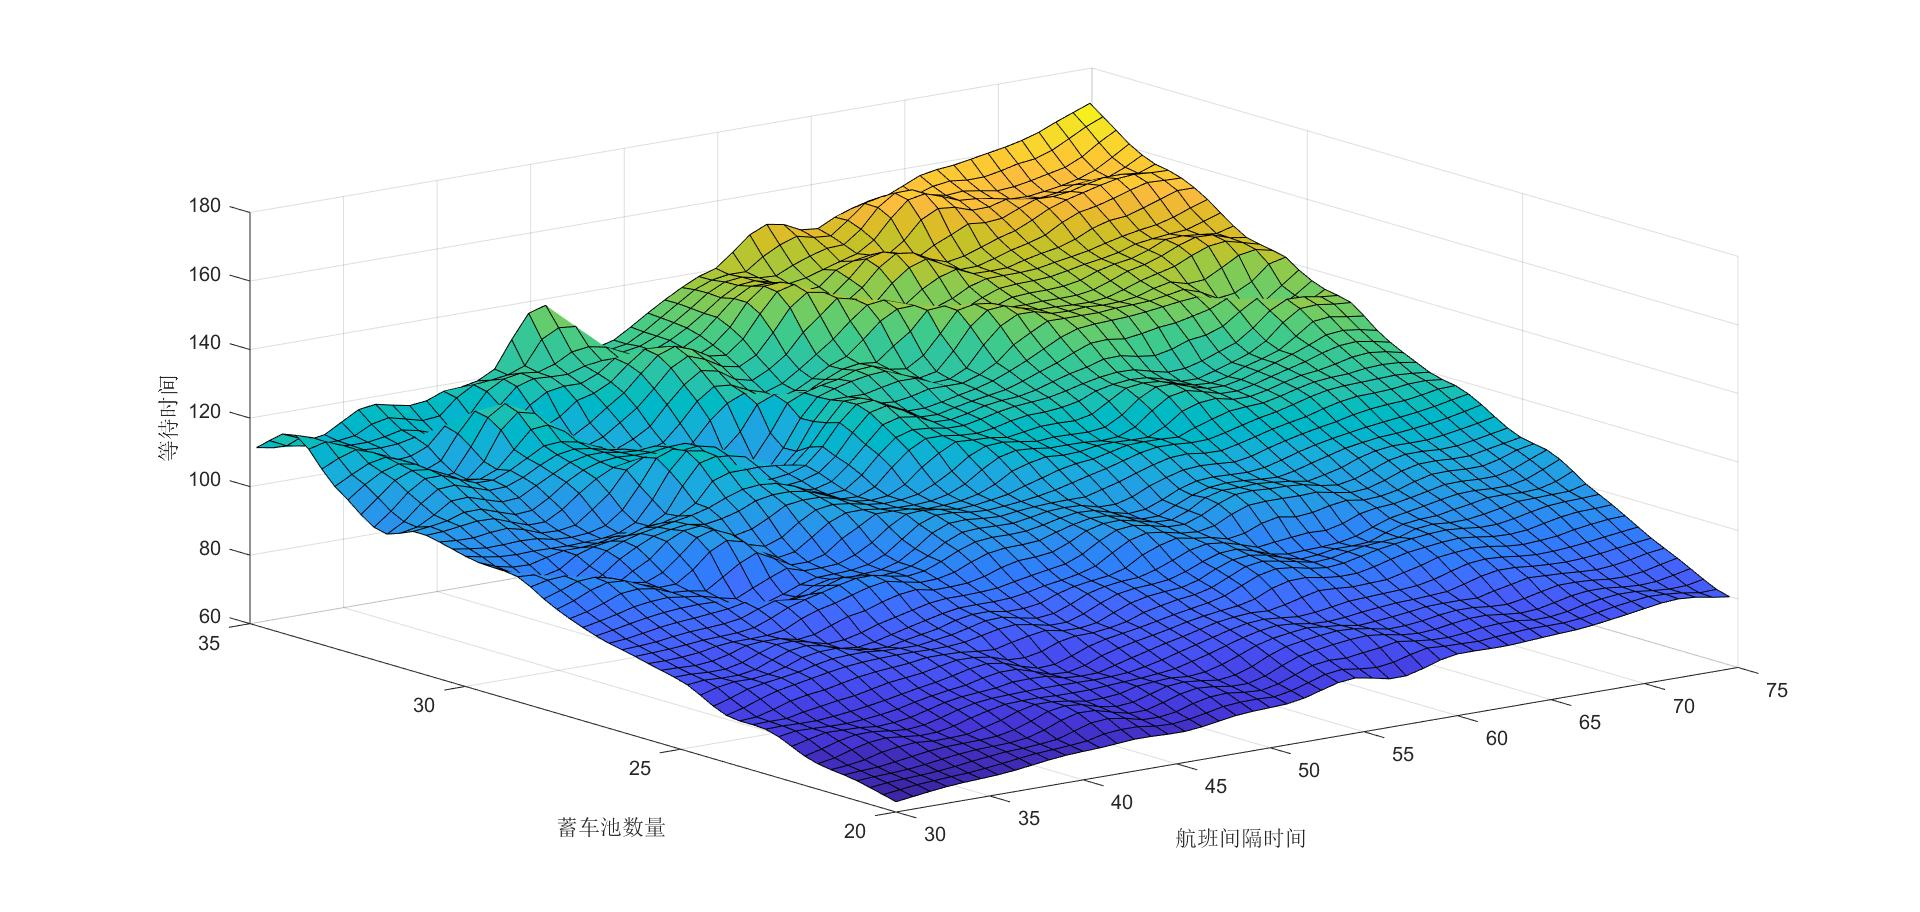
\includegraphics[width=0.8\textwidth]{img/problem2_func.jpg}
		\caption{实际参数下的\waittime$(\mbox{\flightnum,\taxinum})$函数图像}
		\label{fi:problem2func}
	\end{figure}
	\begin{figure}[H]   
		\centering   
		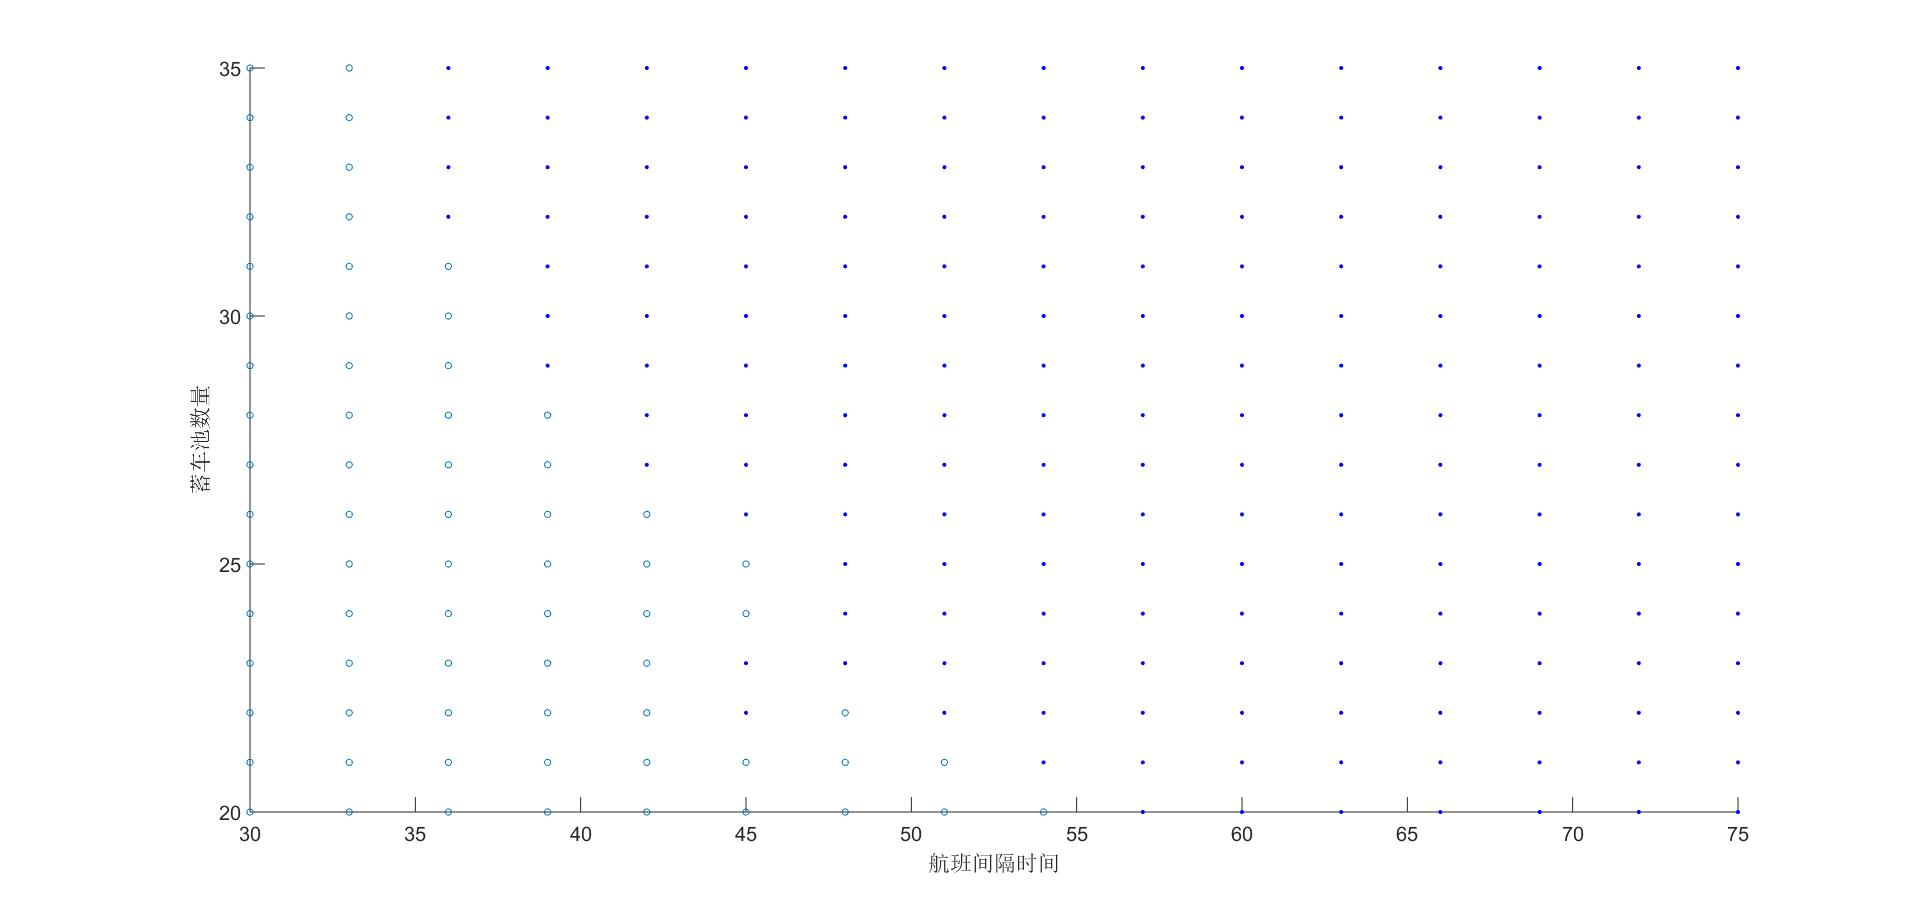
\includegraphics[width=1.0\textwidth]{img/problem2_pred.jpg}   
		\caption{出租车司机决策预测}   
		\label{fi:problem2pred}    
	\end{figure}
	图\ref{fi:problem2func}反映了在不同的\flightnum 和\taxinum 下的$\hat{t_w}$和$t_w$的大小分布情况,图\ref{fi:problem2pred}反应的是在不同的\flightnum 和\taxinum 下,出租车做出的决策的预测是空载返回(实心点)或是进入蓄车池等待载客(空心点)。\par
	根据预测得到的不同\flightnum 和\taxinum 下的$\hat{t_w}$与$t_w$进行比较,计算出模型的相对误差:
	\begin{equation}
		e_1=\frac{\left| \hat{t_w}-t_w\right| }{t_w}\times100\%=10.36\%
	\end{equation}
	由此可以看出,该模型与实际情况的误差在合理范围之内,可以用于预测现实情况下的司机的等待时间。	
\end{enumerate}

\subsection{问题三的解答}

\subsection{问题四的解答}

\section{模型总结}
\subsection{灵敏度分析}
\subsection{模型优点}
\begin{enumerate}
	\item 把模型的优点一一列举出来。
\end{enumerate}

\subsection{模型缺点}
\begin{enumerate}
	\item 把模型的缺点一一列举出来。
\end{enumerate}

\bibliography{ref}

\newpage
\appendix
\textbf{附录}
\section{模型代码}
\subsection{问题一代码}
\begin{lstlisting}
	% 这里放置代码
\end{lstlisting}
\end{document}